Se diseñó el módulo de codificación de codewords para realizar la multiplicación de la información recibida con la matriz $\textbf{G}= {I | B}$. La logica resultante es combinacional y el diseño final queda:

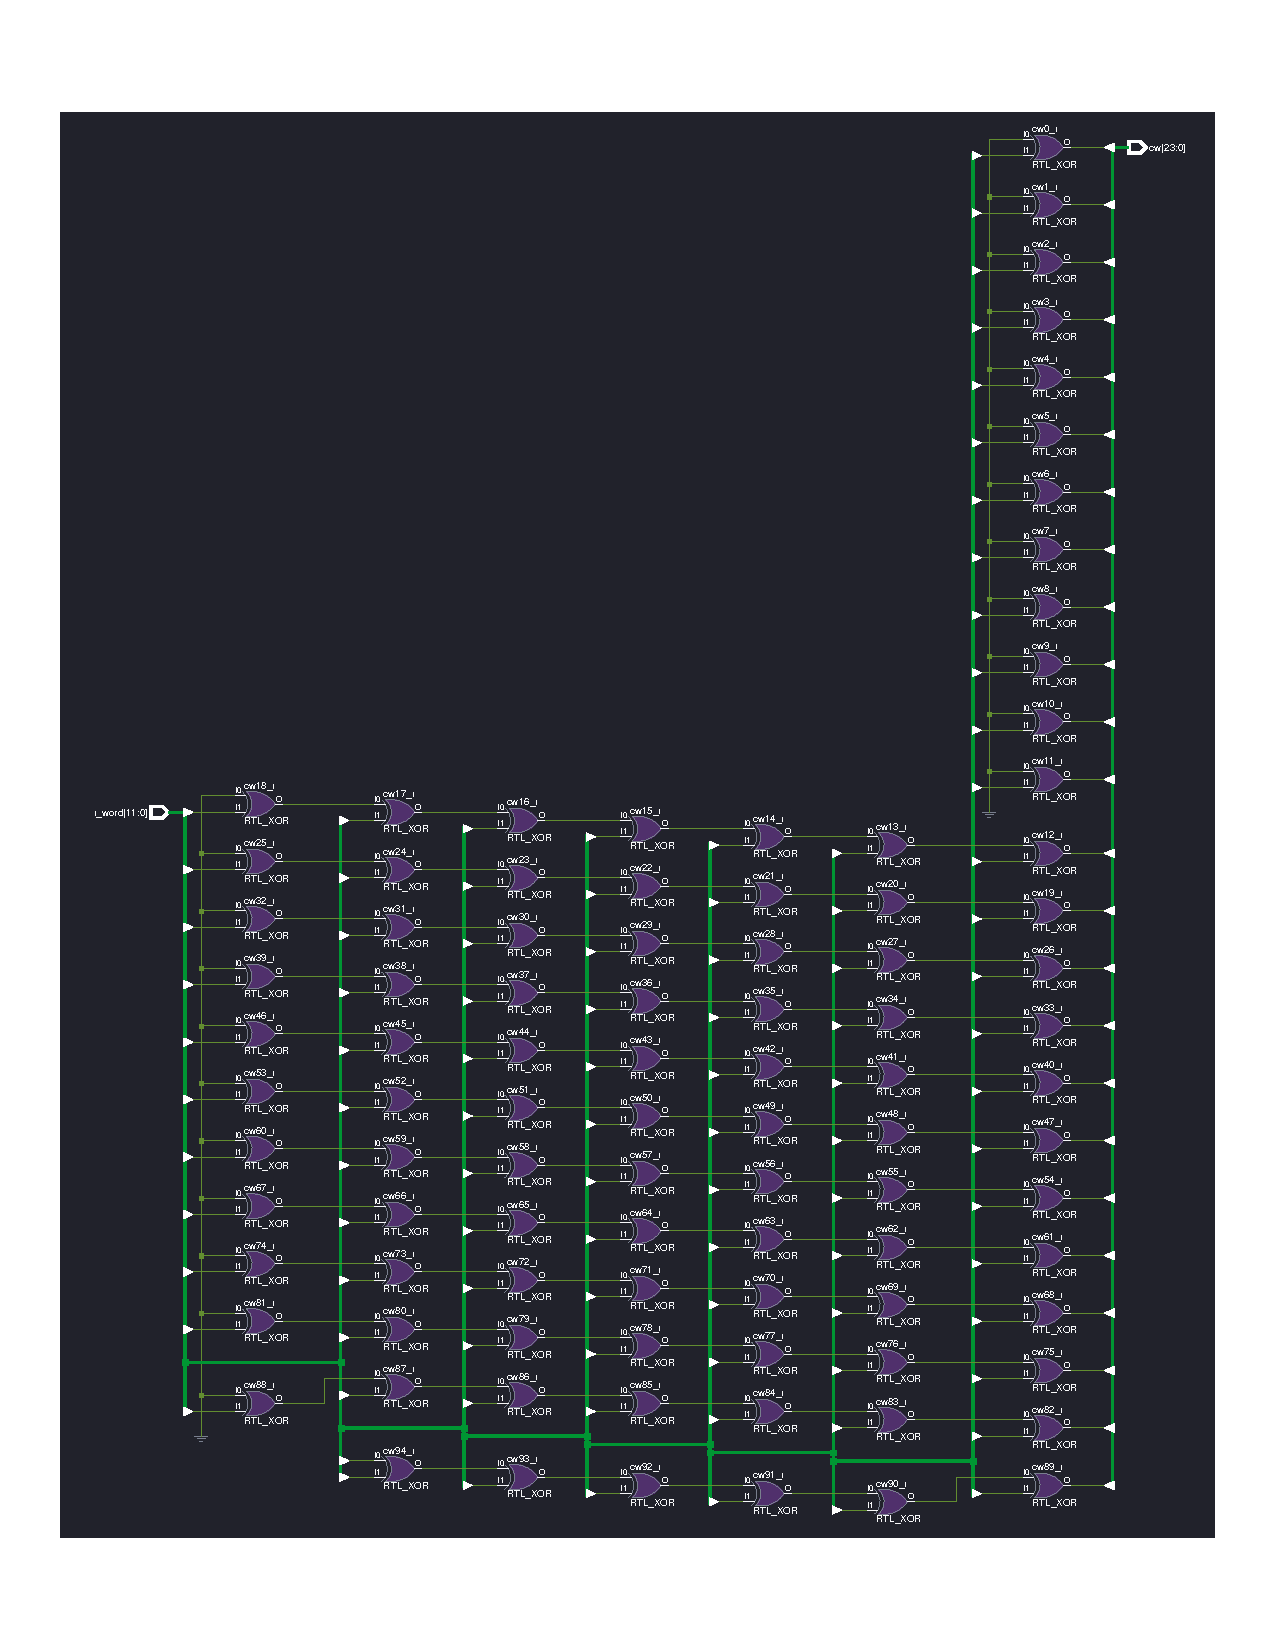
\includepdf[pages=-]{inc/encoder.pdf}

\subsection{Resumen del encoder}
\begin{figure}[H]
    \centering
    \includegraphics[scale=0.3]{encoder-theros1.png}
    % \caption{Implementación RTL del encoder.}
    \label{fig:encoder-theros1}
\end{figure}

\begin{figure}[H]
    \centering
    \includegraphics[scale=0.3]{encoder-theros2.png}
    \caption{Resumen de la implementación RTL del encoder.}
    \label{fig:encoder-theros2}
\end{figure}

\subsection{Validación del encoder}

Se realiza la simulación con el objetivo de verificar la generación de las codewords a partir de las 4096 combinaciones posibles de la palabra de 24-bits a codificar.
Las posibles combinaciones y las codewords resultantes se obtienen del golden model realizado en software.
El formato del archivo es el siguiente: 

\begin{table}[h!]
    \centering
    \begin{tabular}{cc}
        \hline
        \textbf{Columna 1} & \textbf{Columna 2} \\
        \hline
        Información & Codeword \\
        \hline
    \end{tabular}
    %\caption{Información y codeword}
    \label{tab:info-codeword}
\end{table}

Se muestra la simulación realizada en Vivado:

\begin{figure}[h!]
    \centering
    \includegraphics[scale=0.3]{wave-encoder-1.png}
    \caption{Verificación del encoder}
    \label{fig:encoder-theros1}
\end{figure}

Mediante la consola de TCL podemos ver que la implementación en RTL procesa la información correctamente.

\begin{figure}[h!]
    \centering
    \includegraphics[scale=0.3]{verification-encoder.png}
    % \caption{Implementación RTL del encoder.}
    \label{fig:encoder-theros1}
\end{figure}
